\documentclass[12pt]{article}
\usepackage[spanish]{babel}
\usepackage[utf8]{inputenc}
\usepackage{amsmath}
\usepackage{amsfonts}
\usepackage{amssymb}
\usepackage{graphicx}
\usepackage{caption}
\usepackage{subcaption}
\usepackage{hyperref}
\usepackage{doi}
\usepackage{mathtools}
\usepackage{float}
\usepackage[colorinlistoftodos]{todonotes}
\usepackage[letterpaper, margin=1.in]{geometry}
\usepackage[version=3]{mhchem}

\begin{document}

\begin{titlepage}

\newcommand{\HRule}{\rule{\linewidth}{0.5mm}}

\center

\textsc{\LARGE Universidad de los Andes}\\[1.5cm]
\textsc{\Large Departamento de F\'isica}\\[0.5cm]
\textsc{\large Biolog\'ia Sint\'etica}\\[0.5cm] 

\HRule \\[0.4cm]
{ \huge \bfseries \todo{titulo} Proyecto}\\[0.4cm]
\HRule \\[1.5cm]
 

\Large \emph{Autores:}\\
Manuela \textsc{Vanegas Ferro}\\
Juan David \textsc{Estupi\~n\'an M\'endez}\\
Luis Alberto \textsc{Guti\'errez L\'opez}\\[2cm]

\Large \emph{Profesor:}\\
Juan Manuel \textsc{Pedraza Leal}\\[3cm]


{\large Mayo 21 de 2015}\\[2cm]

\vfill

\end{titlepage}

\tableofcontents
\pagebreak

\begin{abstract}
  Your abstract \cite{cleland67}  \cite{harada09a} \cite{engerberg-kulka04}.
\end{abstract}

\section{Introducci\'on}

Existe un mecanismo mediante el cual ciertas especies de plantas al ser atacadas por herbívoros liberan ciertos químicos volátiles que atraen otros insectos que se alimentan de dichos herbívoros \cite{kressler01} \cite{taiz10} \cite{takabayashi96} \cite{turlings95} . Este mecanismo provee una protección tanto directa como indirecta porque, además de atraer insectos predadores de herb\'ivoros, también permiten la comunicación del peligro entre las plantas a largo plazo \cite{kressler01} \cite{taiz10}. En este caso específico, se usarán genes productores de \emph{bergamoteno} de la planta \emph{Nicotiana attenuata} \todo{si?} para atraer insectos del género \emph{Geocoris}, el cual es un predador generalista de aproximadamente 67 especies distintas \cite{crocker80}.\\

El sistema en plantas es lo suficientemente distinguible para que los insectos \emph{Geocoris} detecten la señal por encima de otros olores. Además, el químico es liberado s\'olo cuando hay daños ocasionados por herbivor\'ia, no por daño mec\'anico. Esto se debe a que el sistema es naturalmente activado por la saliva de los herb\'ivoros. Por \'ultimo, la planta env\'ia la se\~nal inmediatamente es atacada por el herb\'ivoro, y en horas del d\'ia en las que los predadores buscan alimento \cite{turlings95}.\\

El \emph{bergamoteno} es un sesquiterpeno que se sintetiza a partir del Farnesyl Difosfato (FPP) mediante la enzima Bergamoteno Sintetasa \cite{sallaud09}. En las plantas, el FPP se produce a partir de dos v\'ias distintas, la v\'ia de DXP y la de Mevalonato \cite{kirby09}, pero esta mol\'ecula no hace parte del metabolismo bacteriano. Por esta raz\'on se han desarrollado numerosos dise\~nos de v\'ias metab\'olicas para producir la mol\'ecula en cantidades significativas en \emph{Escherichia coli} \cite{harada09b}. Un ejemplo de estos dise\~nos es el pl\'asmido pAC-Mev/Scidi/Aacl, el cual contiene las enzimas de la v\'ia del mevalonato hasta la s\'intesis de las dos mol\'eculas precursoras de FPP (ver figura \ref{fig:pac}). Sin embargo, es importante tener en cuenta que el FPP hace parte de una serie de isoprenos que son t\'oxicos para el crecimiento bacteriano \cite{harada09b}. Por esta raz\'on, es vital lograr una fina sincronizaci\'on entre la producci\'on y el uso de esta mol\'ecula.\\

\begin{figure}[H]
  \centering
  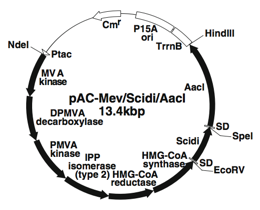
\includegraphics[width=0.5\textwidth]{aaaa.png}
  \caption{\label{fig:pac} Esquema del pl\'asmido pAC-Mev/Scidi/Aacl. Tomado de \cite{harada09b}.}
 \end{figure}


Debido a que este sistema es muy espec\'ifico a ciertas plantas, en este proyecto se busca hacerlo m\'as general, peritiendo que muchas especies de plantas se puedan proteger de una forma m\'as eficiente de los herv\'iboros sin necesidad de usar qu\'imicos insecticidas, los cu\'ales son muy nocivos para el ecosistema \todo{poner mas aqui?}. De esta forma, se busca modificar a la bacteria \emph{Escherichia coli} \todo{hablar de la posibilidad de otras?} para que produzca Bergamoteno cuando ella detecte da\~no por herbivor\'ia. Este proyecto presenta el desafio de controlar la producci\'on de Farnesil pirofosfato (FPP) porque es t\'oxico para \emph{E. coli}, adem\'as se busca optimizar la producci\'on de bergamoteno de tal forma que no sea da\~nino para la planta a largo plazo. \todo{finalmente si?}

\section{Modelo Matem\'atico}
\label{sec:model}
\subsection{Dise\~no}

Para el siguiente modelo cosideramos 2 partes. La primera se refiere a la produce la enzima \emph{Bergamoteno sintetasa} (E en la figura \ref{fig:Circuit}). La otra parte requiere del pl\'asmido \emph{pAC-Mev/Scidi/Aacl}, que sintetiza las enzimas necesarias para llevar \emph{Acetil CoA} a FPP. En el modelo condensamos todos los procesos enzim\'aticos que est\'an mediados por las enzimas para las que el pl\'asmido codifica en un s\'olo proceso enzim\'atico donde el sustrato A presente en la c\'elula reacciona con la enzima Z producida por el pl\'asmido para producir FPP(F en la figura \ref{fig:Circuit}). Ambas partes tienen un promotor activado por la se\~nal de da\~no. Naturalmente el sistema detecta sustancias que producen los herb\'ivoros \todo{citar}, sin embargo, dada la dificultad para encontrar promotores activados por sustancias tan espec\'ificas, se utilizar\'a el promotor \emph{ABRA} que se encuentra en organismos vegetales y est\'a asociado a la recepci\'on y señalizaci\'on de \'acido absc\'icico (ABA) \todo{citar}. Adem\'as, el circuito del pl\'asmido presenta un sitio de inhibici\'on de LacI, el cual es producido por este mismo circuito para generar un feedback negativo. De esta manera, se busca regular la producci\'on de la enzima Z, y as\'i limitar la concentraci\'on de FPP.

\begin{figure}[H]
  \centering
  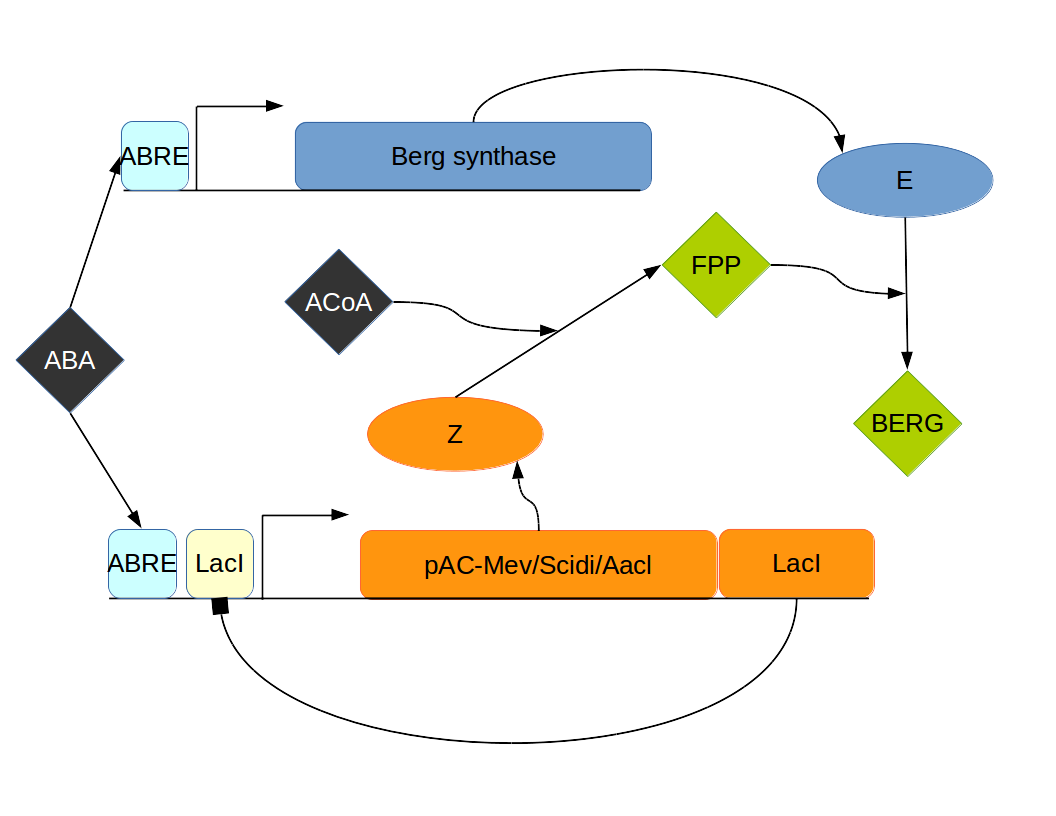
\includegraphics[width=0.5\textwidth]{Circuit.png}
  \caption{\label{fig:Circuit} Interconecciones entre los genes que se van a usar en el modelo.}
\end{figure}

El modelo que se explicar\'a a continuaci\'on tiene como objetivo principal buscar c\'omo se puede producir bergamoteno eficientemente manteniendo al m\'inimo posible la concentraciones de FPP en las c\'elulas.\\

\subsection{Ecuaciones de Hill}

Se model\'o la parte transcripcional como se ha hecho en clase y est\'a explicado en \cite{alon06}. Consideramos que el ADN total del gen a transcribir $\text{D}_{\text{T}}$ es constante, es decir:

\begin{equation} \label{eq:D_T}
[\text{D}_{\text{T}}]=[\text{D}]+[\text{DS}]+[\text{DI}]+[\text{DIS}],
\end{equation}

Donde $[\text{D}]$ representa el ADN libre, $[\text{DIS}]$ el ADN unido tanto al represor I como al activador S, $[\text{DS}]$ el unido al activador, y $[\text{DI}]$ el unido al represor.\\

Para realizar balance detallado se consideraron las siguientes ecuaciones qu\'imicas, las cuales son equivalentes al diagrama del inicio  de la primera tarea del curso.

\begin{align}
\ce{[D] + [S]} &\ce{<=>[\ce{k_{S+}}][\ce{k_{S-}}] [DS]}, \label{eq:rchem1}\\ 
\ce{[D] + [I]} &\ce{<=>[\ce{k_{I+}}][\ce{k_{I-}}] [DI]}, \label{eq:rchem2}\\
\ce{[DS] + [I]} &\ce{ <=>[\ce{k_{I+}}][\ce{k_{I-}}] [DIS]}, \label{eq:rchem3}\\ 
\ce{[DI] + [S]} &\ce{<=>[\ce{k_{S+}}][\ce{k_{S-}}] [DIS]}. \label{eq:rchem4}
\end{align}

Donde las $k$ son las constantes de las respectivas reacciones y se define la constante de disociaci\'on como $K = \frac{k_-}{k_+}$ \cite{alon06}. Seg\'un las ecuaciones qu\'imicas podemos plantear las ecuaciones diferenciales. Al evaluar tiempos mucho mayores a los tiempos en los que ocurre la uni\'on entre el ADN y los factores de transcripci\'on es v\'alido suponer que se ha alcanzado el estado estacionario, obteniendo entonces de las ecuaciones anteriores:

\begin{equation}
\label{eq:Dss}
\dot{[\text{D}]}=0=-k_{S+}[\text{D}][\text{S}]+k_{S-}[\text{DS}]=-k_{I+}[\text{D}][\text{I}]+k_{I-}[\text{DI}],
\end{equation}

De donde se tiene que:

\begin{equation}
\label{eq:K1}
[D][S]=K_S[DS], \quad [D][I]=K_I[DI] 
\end{equation}

Ahora se busca hallar la raz\'on entre el ADN en los distintos estados (dados por la ecuaci\'on \ref{eq:D_T}), se realizar\'a detalladamente para $[DS]$. De la ecuaci\'on \ref{eq:K1} se obtiene:

\begin{equation}
\label{eq:DS}
[D] = \frac{K_S}{S}[DS], \quad [DIS] = \frac{I}{K_I}[DS], \quad [DI]=\frac{K_S}{S}[DIS]=\frac{K_S}{S}\frac{I}{K_I}[DS],
\end{equation}

Para incluir los coeficientes de Hill en el modelo, se realiza el mismo an\'alisis pero considerando la posibilidad de que varias mol\'eculas de los factores de transcripci\'on pueden unirse al ADN, siguiendo el procedimiento del ap\'endice A.2 de \cite{alon06} obtenemos un resultado similar a la ec. \ref{eq:DS}, pero con las fracciones dependientes de S e I elevadas a los coeficientes de Hill $n_S$ y $n_I$, respectivamente. Por lo tanto al reemplazar esto en la ec. \ref{eq:D_T} y reorganizando se tiene que:

\begin{equation}
\frac{[DS]}{[D_T]} = \frac{1}{\left( \frac{K_S}{S} \right)^{n_S} + \left( \frac{I}{K_I} \right)^{n_I} \left( \frac{K_S}{S} \right)^{n_S} + 1 + \left( \frac{I}{K_I} \right)^{n_I}},
\end{equation}

La expresi\'on anterior representa la fracci\'on de ADN ligado a $S$ que hay en equilibrio, al considerar un tiempo suficientemente largo para que ocurran muchos eventos de uni\'on y disociaci\'on de los factores de transcripci\'on esto se puede interpretar como la probabilidad de que el ADN se encuentre en este estado y por lo tanto que la transcripci\'on se d\'e en \'el. As\'i, al multiplicar por la fuerza del promotor $\beta$ obtenemos la tasa de transcripci\'on en dicho estado del ADN.\\

De la misma manera se pueden realizar el an\'alisis para $[DI]$, $[D]$ y $[DIS]$ para obtener las tasas de transcripci\'on en cada uno de los estados. La tasa total es la suma de todas las tasas, donde adem\'as se toma la tasa correspondiente al ADN libre como una constante $\alpha$ correspondiente a la transcripci\'on basal. Tambi\'en se sigue un procedimiento similar para hallar la tasa de producci\'on de $r_E$, que es mucho m\'as sencillo pues s\'olo hay un promotor. Se incluye un t\'ermino de degradaci\'on $\gamma$ tanto de ARN como de prote\'inas y se incluye tambi\'en una tasa de creaci\'on de prote\'inas $k_P$ que tomaremos como constante y se determinar\'a seg\'un el RBS.

Las ecuaciones que se obtienen son las siguientes:

\begin{multline}
\label{eq:rZ}
\dot{r_Z}(t) = 
\alpha_{IS}
+ \frac{\beta_{IS_I}}{\left( \frac{K_I}{I} \right)^{n_I} + 1 + \left( \frac{S}{K_S} \right)^{n_S} \left( \frac{K_I}{I} \right)^{n_I} + \left( \frac{S}{K_S} \right)^{n_S}}\\
+ \frac{\beta_{IS_S}}{\left( \frac{K_S}{S} \right)^{n_S} + \left( \frac{I}{K_I} \right)^{n_I} \left( \frac{K_S}{S} \right)^{n_S} + 1 + \left( \frac{I}{K_I} \right)^{n_I}}
+ \frac{\beta_{IS_{IS}}}{\left( \frac{K_I}{I} \right)^{n_I} \left( \frac{K_S}{S} \right)^{n_S} + \left( \frac{K_S}{S} \right)^{n_S} + \left( \frac{K_I}{I} \right)^{n_I} + 1}
- \gamma_{r_Z} r_Z
\end{multline}

\begin{equation}
\label{eq:Z}
\dot{Z}(t) = k_Z r_Z - \gamma_Z Z
\end{equation}

\begin{multline}
\label{eq:rI}
\dot{r_I}(t) = 
\alpha_{IS}
+ \frac{\beta_{IS_I}}{\left( \frac{K_I}{I} \right)^{n_I} + 1 + \left( \frac{S}{K_S} \right)^{n_S} \left( \frac{K_I}{I} \right)^{n_I} + \left( \frac{S}{K_S} \right)^{n_S}}\\
+ \frac{\beta_{IS_S}}{\left( \frac{K_S}{S} \right)^{n_S} + \left( \frac{I}{K_I} \right)^{n_I} \left( \frac{K_S}{S} \right)^{n_S} + 1 + \left( \frac{I}{K_I} \right)^{n_I}}
+ \frac{\beta_{IS_{IS}}}{\left( \frac{K_I}{I} \right)^{n_I} \left( \frac{K_S}{S} \right)^{n_S} + \left( \frac{K_S}{S} \right)^{n_S} + \left( \frac{K_I}{I} \right)^{n_I} + 1}
- \gamma_{r_I} r_I
\end{multline}

\begin{equation}
\label{eq:I}
\dot{I}(t) = k_I r_I - \gamma_I I
\end{equation}

\begin{equation}
\label{eq:r_E}
\dot{r_E}(t) = \alpha_S + \frac{\beta_S}{1+ \left( \frac{K_S}{S}\right)^{n_S}} - \gamma_{r_E} r_E\\
\end{equation}

\begin{equation}
\label{eq:E}
\dot{E}(t) = k_E r_E - \gamma_EE
\end{equation}

\subsection{Reacciones enzim\'aticas}

Seg\'un la figura \ref{fig:Circuit}, las ecuaciones qu\'imicas de las reacciones entre enzima y sustrato son las siguientes

\begin{align}
\ce{[Z] + [A]} &\ce{<=>[\ce{\hat{k}_+}][\ce{\hat{k}_-}] [ZA] ->[\ce{\hat{k}_{cat}}] [Z] + [F]}, \label{eq:echem1}\\
\ce{[E] + [F]} &\ce{<=>[\ce{k_+}][\ce{k_-}] [EF] ->[\ce{k_{cat}}] [E] + [B]}, \label{eq:echem2}
\end{align}

donde [Z] y [E] son las enzimas que proceden del pl\'asmido y la bergamoteno sintetasa, respectivamente. [F] y [B] corresponden a FPP y el bergamoteno. Con las ecuaciones \ref{eq:echem1} y \ref{eq:echem2}, se obtubieron las ecuaciones diferenciales para el FPP y el Bergamoteno, siguiendo el siguiente razonamiento.\\
Debido a que el Acetil CoA, el sustrato de la enzima que produce FPP, proviene del metabolismo constante de la bacteria, se puede suponer que su concentraci\'on $[A]$ es constante y elevada. Por lo tanto, para la producci\'on de FPP habr\'a un t\'ermino positivo que sigue las ecuaciones de Michaelis-Menten.\\
Por otra parte, debido a que el FPP est\'a siendo consumido a la vez para producir Bergamoteno, se requiere un t\'ermino negativo en la ecuaci\'on diferencial que ilustre este proceso. Sin embargo, se usa la aproximaci\'on de la ecuaci\'on de velocidad cuadr\'atica ilustrado en \cite{chemwiki1}. Esta ecuaci\'on es v\'alida cuando la concentraci\'on de sustrato no es constante y es similar a la concentraci\'on de la enzima que cataliza dicho sustrato \cite{chemwiki1}. Dicho esto, las ecuaciones que se usar\'an son

\begin{eqnarray}
\dot{F} &=& \frac{K_{\text{cat1}}[Z][A]}{K_{\text{M1}}+[A]} - K_{\text{cat2}}\frac{J-\sqrt{J^2-4[E][F]}}{2} \label{eq:DiffF}\\
\dot{B} &=& K_{\text{cat2}}\frac{J-\sqrt{J^2-4[E][F]}}{2} - \gamma_B [B] \label{eq:DiffB}\\
\text{Donde} && J=[E]+[F]+K_{\text{M2}} \nonumber
\end{eqnarray}

Y $K_{M1}$, $K_{\text{cat}1}$, $K_{M2}$, $K_{\text{cat}2}$, son las constantes de las enzimas del pl\'asmido y de la bergamoteno sintetasa, respectivamente. $\gamma_B$ es el t\'ermino introducido por el decaimiento del Bergamoteno debido a la difusi\'on y divisi\'on celular. Este t\'ermino no es inclu\'ido en la ecuaci\'on para F pues esta sustancia es utilizada en otra reacci\'on enzim\'atica que ocurre mucho m\'as r\'apido que el tiempo de degradaci\'on de las prote\'inas.\\

Las ecuaciones diferenciales para F y B (\ref{eq:DiffF} y \ref{eq:DiffB}) dependen de las cantidades calculadas con el modelo estoc\'astico para la producci\'on de las enzimas, estas cantidades siguen la din\'amica ilustrada en la secci\'on anterior.\\

Las ecuaciones \ref{eq:rZ} - \ref{eq:E}, \ref{eq:DiffF} y \ref{eq:DiffB}, junto con las condiciones iniciales para cada una, constituyen el sistema de ecuaciones que ser\'a simulado mediante los programas.

\subsection{Par\'ametros}

En la tabla \ref{tab:1} est\'an listados los par\'ametros del modelo.

\begin{table}[H]
\centering
\begin{tabular}{c c c c c} 
 \hline
 S\'imbolo & Valor & Unidades & Descripci\'on & Ref. \\
 \hline\hline
 W & 1791/RFP & - & Mutaci\'on en el promotor constitutivo & BBa\_J23113 \\
 $\alpha_S$ & $1.53/W$ & - & Actividad basal de S & Kelly  2009  \\ 
 $\beta_S$ & $51.2 \alpha_S$ & - &  Actividad de S con ABA & Hobo 1999 \\
 $\alpha_{RS}$ & $1.53/W$ & - & Actividad basal de RS & Kelly  2009\\
 $\beta_{RS_R}$ & $\alpha_{RS}/620$ & - & Actividad de RS con LacI & Lutz 1997\\
 $\beta_{RS_S}$ & $51.2 \alpha_{RS}$ & - & Actividad de  RS con ABA & Hobo 1999\\
 $\beta_{RS_RS}$ & $\beta_{RS_R}$ & - & Actividad de RS con ABA y LacI & Bujard 1997 \\
 $K_S$ & * &  & Constante de disociaci\'on del ABA-ABRE &  \\
 $n_S$ & * &  & Coeficiente de Hill de S & \\
 $k_E$ & * &  & Tasa de traducci\'on de E &   \\
 $K_R$ & $8*10^{-4}$ & mM & Constante de disociaci\'on de LacI & Basu 2005\\
 $n_R$ & 1 & - & Coeficiente de Hill de LacI & Kalisky 2007\\
 $k_R$ & * & & Tasa de traducci\'on de R & \\
 $\gamma_R$ & * & & Tasa de degradaci\'on de la enzima Z & \\
 $\gamma_E$ & 1/30 & $min^{-1}$ & Tasa de degradaci\'on del ARN (de E y R) & \\
 $K_{MBerg}$ & 0.0014 & $mM$ & Constante de MM para enzima E & Jones 2007 \\
 $K_{CBerg}$ & 0.34 & $s^{-1}$ & Turnover para enzima E & Jones 2007 \\
 $K_{MFpp}$ & 0.0048 & $mM$ & Constante de MM para enzima Z & Kittleman 2007 \\
 $K_{CFpp}$ & 0.34 & $s^{-1}$ & Turnover para enzima Z & Kittleman 2007 \\
 \hline
\end{tabular}
\caption{Par\'ametros del modelo. S hace referencia al promotor \emph{ABRA} individual y RS al promotor \emph{ABRA} con el sitio de \emph{lacI}. Las tasas de degradaci\'on $\gamma$ se tomaron iguales en todos los casos.}
\label{tab:1}
\end{table}

\subsection{Modelos determinista y estoc\'astico}

Para realizar la simulaci\'on estoc\'astica se utiliz\'o el algoritmo de Gillespie. Si los eventos de producci\'on de ARN y prote\'inas son considerados separadamente se tendr\'ian 8 eventos, lo cual tomar\'ia mucho tiempo en ejecutar. Por lo tanto, se realiz\'o el algoritmo con r\'afagas de prote\'inas, de tal forma que al evento de producirse un RNA, se producen $\frac{k_P}{\gamma_r}$ prote\'inas. Esto es lo que corresponde al promedio de prote\'inas que se pueden traducir de un RNA durante su tiempo de vida.\\

Por otra parte, las escalas de tiempo a las que ocurren las reacciones enzim\'aticas son mucho menores a las de la producci\'on de RNA y prote\'inas, por lo tanto los efectos del ruido son despreciables en ellas y por lo tanto se pueden resolver de manera determinista. Se utiliz\'o en este caso el m\'etodo Runge-Kutta de Cuarto Orden.\\

En programa fu\'e realizado utilizado IPython notebook, se puede ver el c\'odigo fuente en el ap\'endice \ref{sec:code}.

\subsection{An\'alisis de sensibilidad}
Se realiz\'o un an\'alisis de sensibilidad usando las constantes que no se conocen. \'Estas se pueden dividir en 2 grupos, $W$ y $\gamma_R$ que son manipulables y $K_S$, $n_S$, $k_E$ y $k_R$ que son las que queremos optimizar. A partir de esto, se seleccionaron 3 niveles distintos para $W$ y $\gamma_R$, y 4 niveles posibles para las dem\'as. Para escoger el r\'ango \'optimo, se estableci\'o que la concentraci\'on de FPP m\'axima no pod\'ia superar los $0.0004 mM$ y que el nivel de bergamoteno prodicido fuera el m\'aximo. Esto se justifica porque no queremos una cantidad de FPP que llegue a ser t\'oxica muy r\'apidamente, y queremos la mayor cantidad posible de bergamoteno.\\

\begin{figure}[H]
  \begin{subfigure}[b]{0.5\textwidth}
  	\centering
  	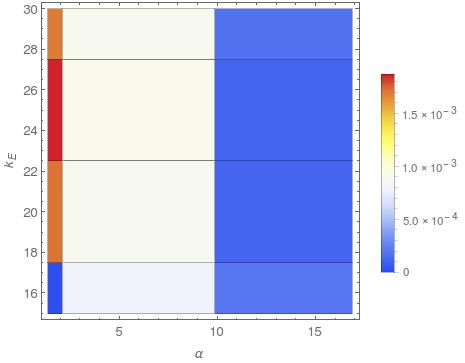
\includegraphics[width=\textwidth]{alpha-kE.jpeg}
  	\caption{\label{fig:alpha-kE} Barrido para $\alpha$ y $k_E$.}
  \end{subfigure}
  \begin{subfigure}[b]{0.5\textwidth}
  	\centering
  	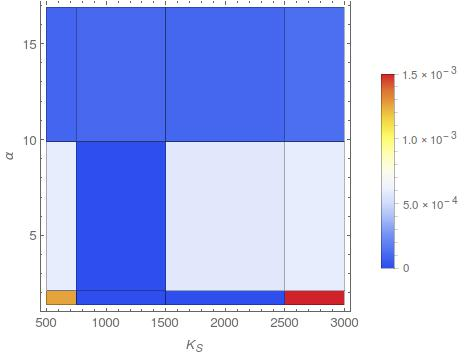
\includegraphics[width=\textwidth]{alpha-KS.jpeg}
  	\caption{\label{fig:alpha-kS} Barrido para $\alpha$ y $K_S$.}
  \end{subfigure}
    
  \begin{subfigure}[b]{0.5\textwidth}
	\centering
  	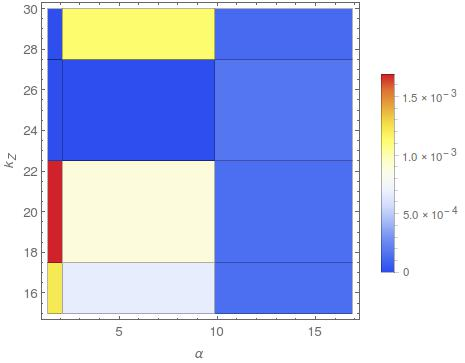
\includegraphics[width=\textwidth]{alpha-kz.jpeg}
  	\caption{\label{fig:alpha-kz} Barrido para $\alpha$ y $k_Z$.}
  \end{subfigure}  
  \begin{subfigure}[b]{0.5\textwidth}
  	\centering
  	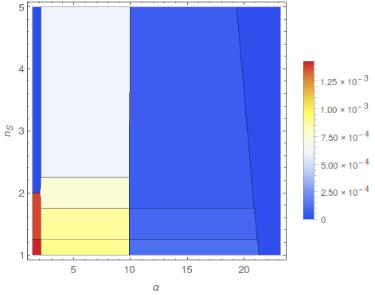
\includegraphics[width=\textwidth]{alpha-nS.jpeg}
  	\caption{\label{fig:alpha-nS} Barrido para $\alpha$ y $n_S$.}
  \end{subfigure}  
\caption{\label{fig:alpha} an\'alisis para $\alpha$} 
\end{figure}

\begin{figure}[H]
	\begin{subfigure}[b]{0.5\textwidth}
  		\centering
  		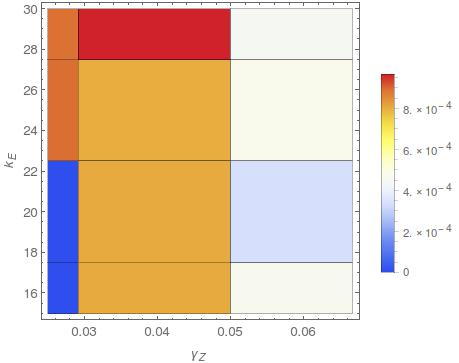
\includegraphics[width=\textwidth]{gammaZ-kE.jpeg}
  		\caption{\label{fig:gammaZ-kE} Barrido para $\gamma_Z$ y $k_E$.}
  	\end{subfigure}
	\begin{subfigure}[b]{0.5\textwidth}
		\centering
  		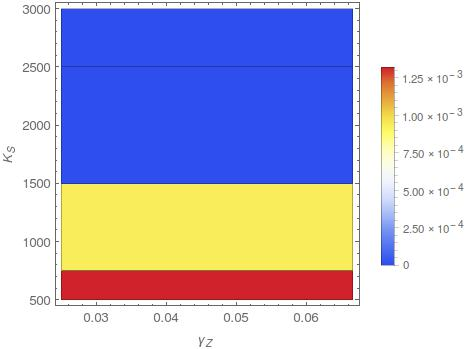
\includegraphics[width=\textwidth]{gammaZ-KS.jpeg}
		\caption{\label{fig:gammaZ-KS} Barrido para $\gamma_Z$ y $K_S$.}
  	\end{subfigure} 	
  	
  	\begin{subfigure}[b]{0.5\textwidth}
		\centering
		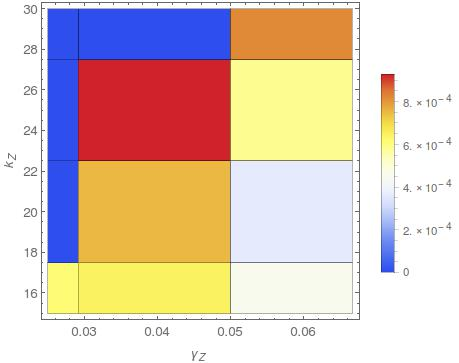
\includegraphics[width=\textwidth]{gammaZ-kZ.jpeg}
		\caption{\label{fig:gammaZ-kZ} Barrido para $\gamma_Z$ y $k_Z$.}
  	\end{subfigure} 	
  		\begin{subfigure}[b]{0.5\textwidth}
		\centering
		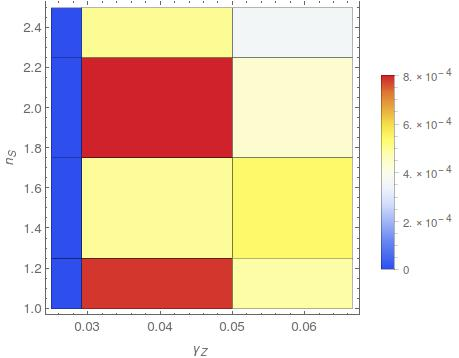
\includegraphics[width=\textwidth]{gammaZ-nS.jpeg}
		\caption{\label{fig:gammaZ-nS} Barrido para $\gamma_Z$ y $n_S$.}
  	\end{subfigure} 	
 \caption{\label{fig:gammaZ} an\'alisis para $\gamma _Z$}	
 \end{figure}

Se puede observar que para valores intermedios de $W$ (\ref{fig:alpha}) y de $\gamma _Z$ (\ref{fig:gammaZ}) se obtienen los valores m\'as estables para las diferentes combinaciones de las dem\'as constantes. Hay que recordar que $W$ est\'a relacionado inversamente con la producci\'on basal de RNA tanto para los circuitos del p\'lasmido como para los de la enzima del bergamoteno.

\appendix
\section{Ap\'endices}
\subsection{C\'odigo fuente de la simulaci\'on}
\label{sec:code}

\bibliographystyle{plain}
\bibliography{written.bib}

\end{document}
